\documentclass[dvipsnames, 10pt, table]{beamer}
\usepackage{graphicx}
\usepackage{listings}
\usepackage{xcolor}
\usepackage[
  backend=bibtex,
  style=ieee,
  sorting=ydnt
  ]{biblatex}
\usepackage[edges]{forest}
\addbibresource{quotes.bib}

\lstset{basicstyle=\footnotesize\ttfamily,
        keywordstyle=\footnotesize\color{blue}\ttfamily}

\lstdefinestyle{tssg}{
  %belowcaptionskip=1\baselineskip,
  %breaklines=true,
  %frame=L,
  %xleftmargin=\parindent,
  showstringspaces=false,
  keywordstyle=\bfseries\color{green!40!black},
  morekeywords={let, node, attr, edge, "=", "->"},
  identifierstyle=\color{blue},
  stringstyle=\color{orange},
}

\lstdefinestyle{yaml}{
  keywordstyle=\bfseries\color{green!40!black},
  morekeywords={nodes, edges, filepaths, name, kind, source, sink},
  % identifierstyle=\color{cyan},
}

\definecolor{PastelGreen}{HTML}{1A7A67}
\definecolor{PastelBlue}{HTML}{2C3E50}
\definecolor{PastelWhite}{HTML}{FAF8F6}
\definecolor{PastelLilac}{HTML}{A391C1}
\definecolor{PastelRed}{HTML}{FAA0A0}

\definecolor{TrenordBlue}{HTML}{006297}
\definecolor{TrenordLightGreen}{HTML}{b6dd79}
\definecolor{TrenordDarkGreen}{HTML}{79be20}
\definecolor{TrenordFalseGreen}{HTML}{d6e965}

\definecolor{FERRed}{HTML}{d9585d}
\definecolor{FERDarkGreen}{HTML}{369389}
\definecolor{FERLightGreen}{HTML}{44a25a}

\definecolor{ATMRed}{HTML}{ef1a2f}
\definecolor{ATMGreen}{HTML}{5d982e}
\definecolor{ATMYellow}{HTML}{fdb90b}
\definecolor{ATMBlue}{HTML}{14386a}
\definecolor{ATMLilac}{HTML}{9a8fc5}

\definecolor{XMPRGreen}{HTML}{00685e}
\definecolor{XMPRBlue}{HTML}{003da5}
\definecolor{XMPRGray}{HTML}{474b4e}

\usetheme{Madrid}

%% FER
% \setbeamercolor{palette primary}{bg=FERDarkGreen,fg=white}
% \setbeamercolor{author in head/foot}{bg=FERLightGreen,fg=black}
% \setbeamercolor{title in head/foot}{bg=FERRed,fg=black}
% \setbeamercolor{date in head/foot}{bg=FERDarkGreen,fg=black}

%% TRENORD
\setbeamercolor{palette primary}{bg=TrenordBlue,fg=white}
\setbeamercolor{author in head/foot}{bg=TrenordLightGreen,fg=black}
\setbeamercolor{title in head/foot}{bg=TrenordDarkGreen,fg=black}
\setbeamercolor{date in head/foot}{bg=TrenordFalseGreen,fg=black}

%% ATM
% \setbeamercolor{palette primary}{bg=ATMGreen,fg=white}
% \setbeamercolor{author in head/foot}{bg=ATMRed,fg=black}
% \setbeamercolor{title in head/foot}{bg=ATMYellow,fg=black}
% \setbeamercolor{date in head/foot}{bg=ATMLilac,fg=black}

%% XMPR
% \setbeamercolor{palette primary}{bg=XMPRGreen,fg=white}
% \setbeamercolor{author in head/foot}{bg=XMPRBlue,fg=white}
% \setbeamercolor{title in head/foot}{bg=XMPRBlue,fg=white}
% \setbeamercolor{date in head/foot}{bg=XMPRBlue,fg=white}
% \setbeamercolor{structure}{fg=XMPRGray}

% \usecolortheme[named=PastelBlue]{structure}

\date[6 November 2025]{}

\title[TSD Seminary]{A Language-Agnostic Framework for Dependency Graph Construction}
\subtitle{}
% \author{Refolli~F.~865955}
\author[Francesco~Refolli]{Francesco~Refolli}
\logo{
\includegraphics[height=2.5cm]{logo_unimib.pdf}}

\newcommand{\putimage}[2] {
  \begin{figure}[H]
    \centering
    \includegraphics[width=#2\linewidth]{#1}
	\end{figure}
}

\newcommand{\putimagecouple}[4] {
  \begin{figure}[!htb]
    \centering
    \begin{minipage}{0.45\linewidth}
      \centering
      \includegraphics[width=\linewidth]{#1}
      \caption{#2}
    \end{minipage}
    \hspace{0.25cm}
    \begin{minipage}{0.45\linewidth}
      \centering
      \includegraphics[width=\linewidth]{#3}
      \caption{#4}
    \end{minipage}
  \end{figure}
}

\begin{document}

\frame{\titlepage}

\begin{frame}
\frametitle{Outline}
\tableofcontents
\end{frame}

\setbeamertemplate{logo}{}

\section{Assessing Software Quality}
\begin{frame}
  \centering
  \Huge
  Assessing Software Quality
\end{frame}

\begin{frame}
  \frametitle{Architectural Smells}
  \begin{definition}
    An \textbf{architectural smell} is a sign of poor design choices on the architectural level.
  \end{definition}

  \begin{itemize}
    \item Similar to the more known Code Smells.
    \item They can be detected by analyzing code shape, components and the dependency graph.
    \item The presence of many smells in a software project increases the estimate of \textbf{Technical Debt}, which indicates the future cost of maintenance, development and evolution.
    \item By Lehman's laws of software evolution we can expect it to grow over time, as bad practises effects stratify
  \end{itemize}
\end{frame}

\begin{frame}
  \frametitle{God Component}
  \begin{columns}
    \begin{column}{0.5\textwidth}
      \begin{figure}
        \begin{center}
          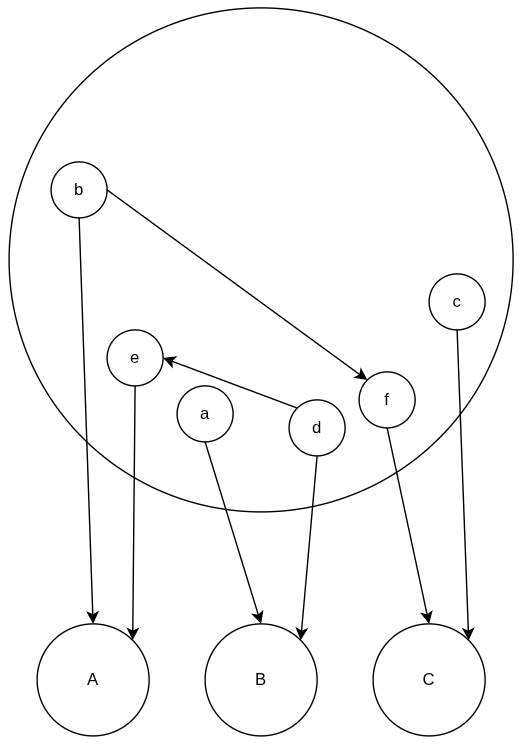
\includegraphics[width=0.8\textwidth]{figures/architectural-smells/god-component.png}
        \end{center}
      \end{figure}
    \end{column}
    \begin{column}{0.5\textwidth}
      \begin{itemize}
        \item One big component with a lot of heterogeneous sub-components inside
        \item Probably takes care of a lot of different concerns
        \item Probably has a lot of outwards dependencies and a few inwards dependencies
        \item Probably is a consistent percentage of the code
        \item Typical of Legacy Systems (especially \textbf{monolithic} architectures)
      \end{itemize}
    \end{column}
  \end{columns}
\end{frame}

\begin{frame}
  \frametitle{Deep Hierarchy}
  \begin{columns}
    \begin{column}{0.5\textwidth}
      \begin{figure}
        \begin{center}
          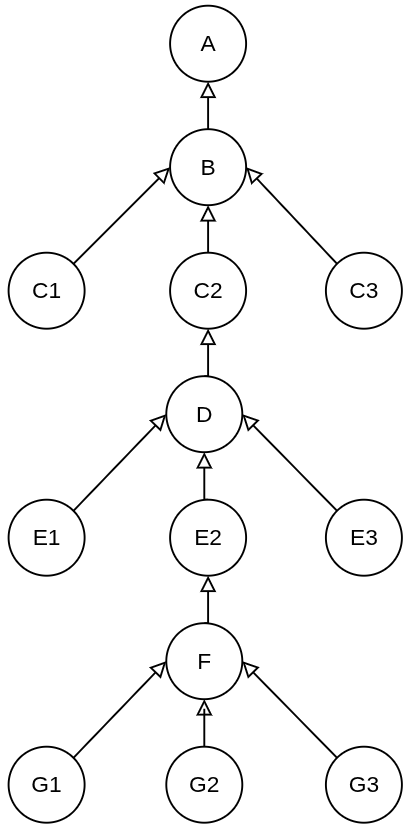
\includegraphics[width=0.6\textwidth]{figures/architectural-smells/deep-hierarchy.png}
        \end{center}
      \end{figure}
    \end{column}
    \begin{column}{0.5\textwidth}
      \begin{itemize}
        \item A long inheritance chain, each level adding a bit of behaviour
        \item Suggests high implementation sparsity
        \item Suggests abuse/loss of generalization
        \item Typical of Object-Oriented Programming
      \end{itemize}
    \end{column}
  \end{columns}
\end{frame}

\begin{frame}
  \frametitle{Wide Hierarchy}
  \begin{columns}
    \begin{column}{0.5\textwidth}
      \begin{figure}
        \begin{center}
          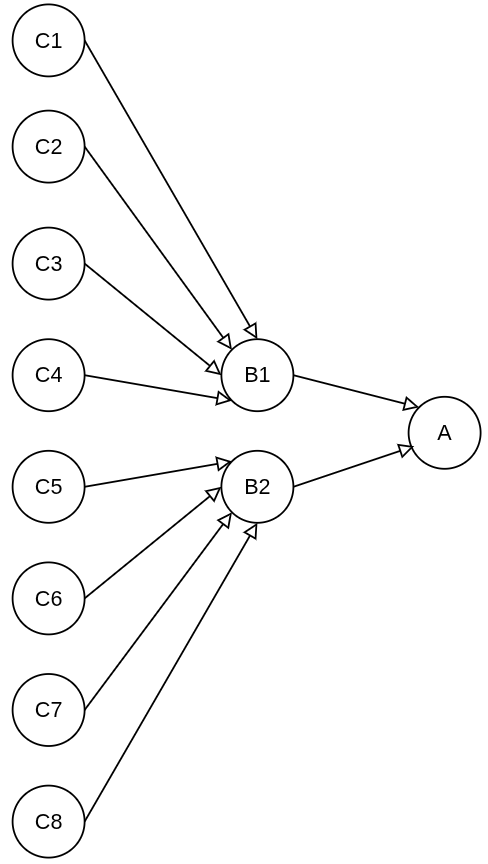
\includegraphics[width=0.7\textwidth]{figures/architectural-smells/wide-hierarchy.png}
        \end{center}
      \end{figure}
    \end{column}
    \begin{column}{0.5\textwidth}
      \begin{itemize}
        \item A hierarchy chain with at each level many children
        \item Suggests high implementation sparsity
        \item Suggests abuse/loss of generalization
        \item Typical of Object-Oriented Programming
      \end{itemize}
    \end{column}
  \end{columns}
\end{frame}

\begin{frame}
  \frametitle{Cyclic Hierarchy}
  \begin{columns}
    \begin{column}{0.5\textwidth}
      \begin{figure}
        \begin{center}
          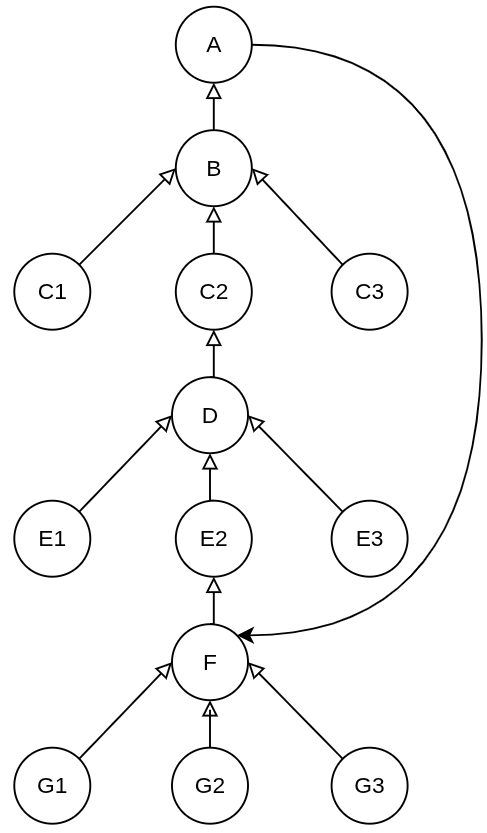
\includegraphics[width=0.7\textwidth]{figures/architectural-smells/cyclic-hierarchy.png}
        \end{center}
      \end{figure}
    \end{column}
    \begin{column}{0.5\textwidth}
      \begin{itemize}
        \item Like the previous, but with a twist
        \item A parent component is actively depending on a child component
        \item Suggests a short-circuit of abstractions
        \item Typical of Object-Oriented Programming
      \end{itemize}
    \end{column}
  \end{columns}
\end{frame}

\begin{frame}
  \frametitle{Unstable Dependency}
  \begin{columns}
    \begin{column}{0.5\textwidth}
      \begin{figure}
        \begin{center}
          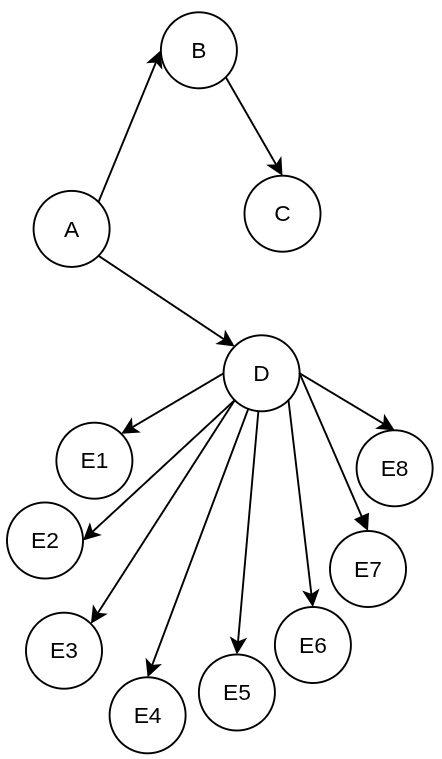
\includegraphics[width=0.7\textwidth]{figures/architectural-smells/unstable-dependency.png}
        \end{center}
      \end{figure}
    \end{column}
    \begin{column}{0.5\textwidth}
      \begin{itemize}
        \item A stable component depending on a unstable component
        \item (In)stability is usually defined by the ratio $\frac {Ce} {Ca + Ce}$
        \item Such a component is difficult to maintain stable because its dependencies have a lot of reasons to change for
      \end{itemize}
    \end{column}
  \end{columns}
\end{frame}

\begin{frame}
  \frametitle{Cyclic Dependency}
  \begin{columns}
    \begin{column}{0.5\textwidth}
      \begin{figure}
        \begin{center}
          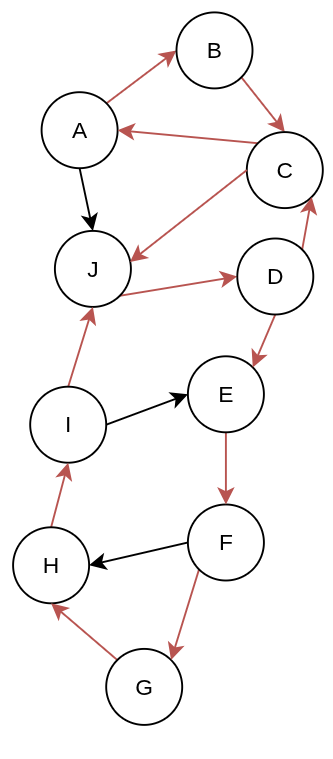
\includegraphics[width=0.55\textwidth]{figures/architectural-smells/cyclic-dependency.png}
        \end{center}
      \end{figure}
    \end{column}
    \begin{column}{0.5\textwidth}
      \begin{itemize}
        \item Components involved in a cycle are difficult to change
        \item Typical of legacy systems
      \end{itemize}
    \end{column}
  \end{columns}
\end{frame}

\begin{frame}
  \frametitle{Hub-Like Dependency}
  \begin{columns}
    \begin{column}{0.5\textwidth}
      \begin{figure}
        \begin{center}
          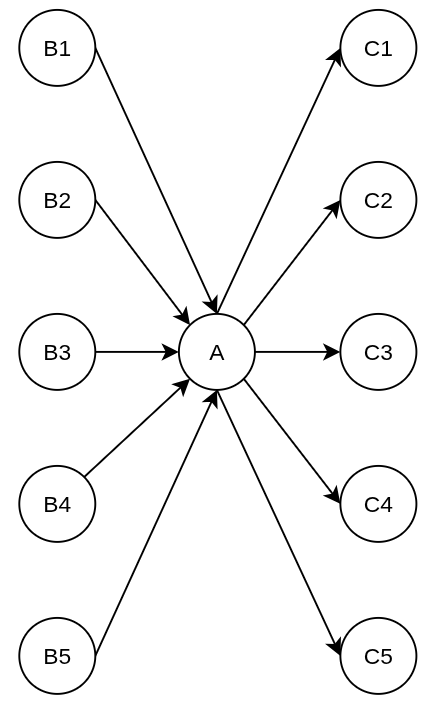
\includegraphics[width=0.7\textwidth]{figures/architectural-smells/hub-like-dependency.png}
        \end{center}
      \end{figure}
    \end{column}
    \begin{column}{0.5\textwidth}
      \begin{itemize}
        \item A component with a lot of inwards and outwards dependencies
        \item To stable to allow for changes
        \item Too unstable to depend on
        \item Typical of many legacy library components
      \end{itemize}
    \end{column}
  \end{columns}
\end{frame}

\begin{frame}
  \frametitle{Arcan}
  \begin{figure}
    \begin{center}
      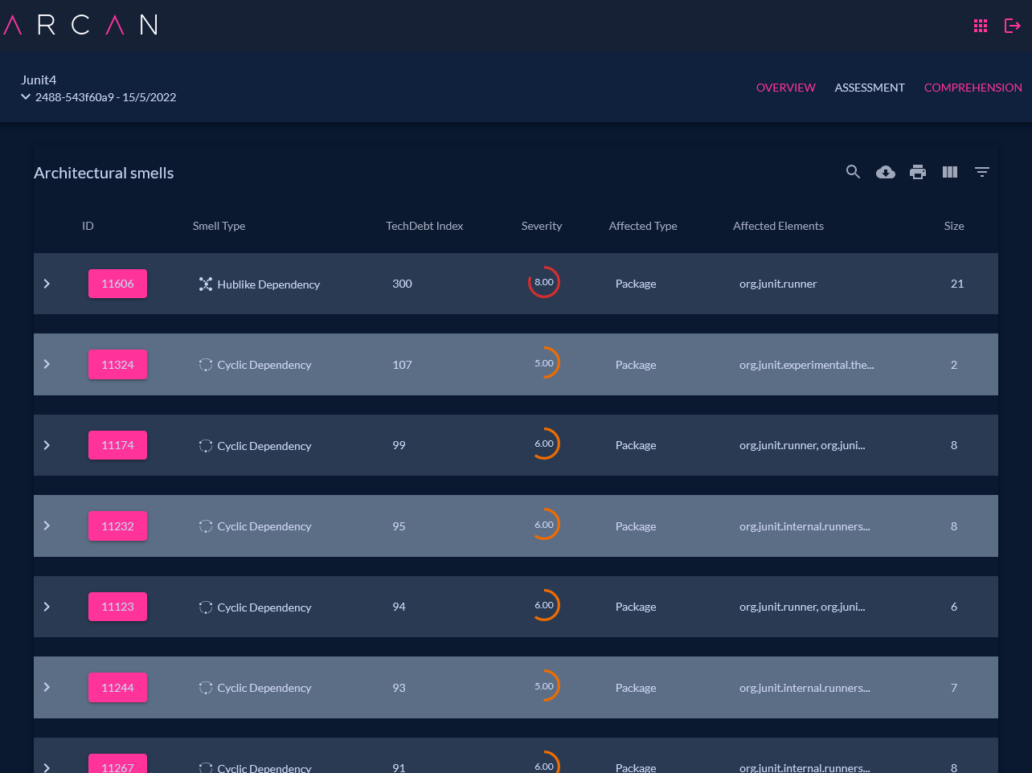
\includegraphics[width=0.85\textwidth]{figures/architectural-smells/arcan-list.png}
    \end{center}
  \end{figure}
\end{frame}

\begin{frame}
  \frametitle{The Dependency Graph}
  \begin{figure}
    \begin{center}
      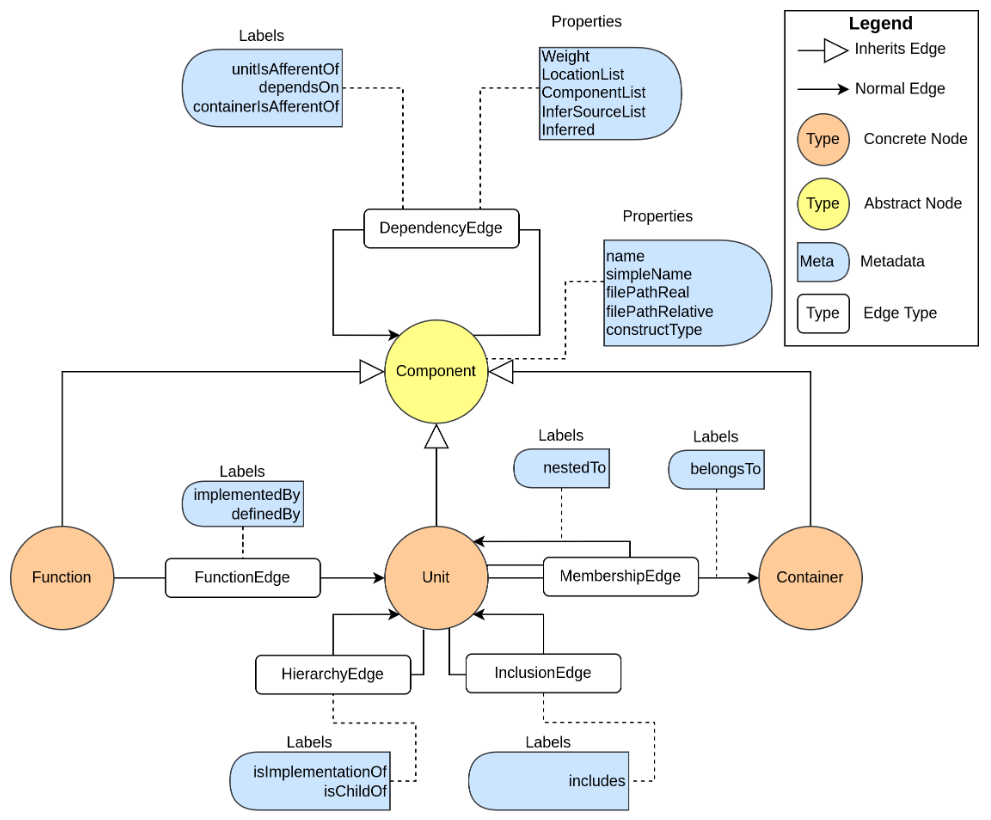
\includegraphics[width=0.7\textwidth]{figures/architectural-smells/arcan-dep-graph.png}
    \end{center}
  \end{figure}
\end{frame}

\begin{frame}
  \frametitle{The Architectural Smell Graph}
  \begin{figure}
    \begin{center}
      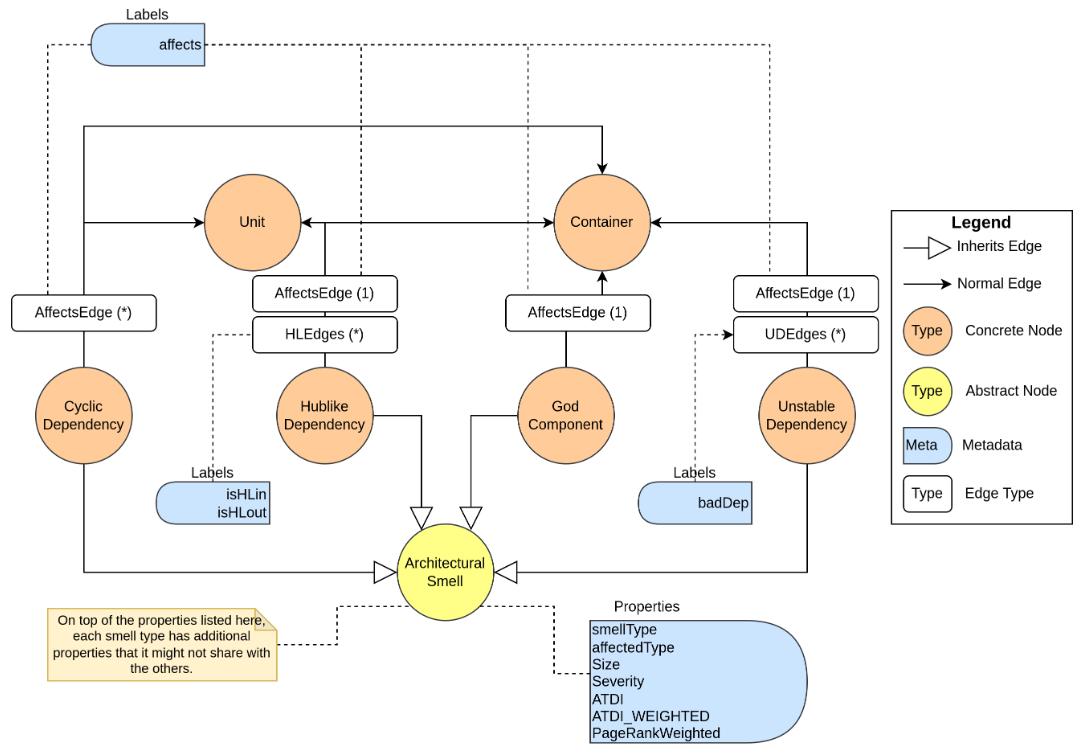
\includegraphics[width=0.8\textwidth]{figures/architectural-smells/arcan-smell-graph.png}
    \end{center}
  \end{figure}
\end{frame}

\section{The "Tower of Babel" Problem}
\begin{frame}
  \centering
  \Huge
  The "Tower of Babel" Problem
\end{frame}

\begin{frame}
  \frametitle{Language Segmentation}
  Computing language usage shares is not easy ...
  \begin{columns}
    \begin{column}{0.5\textwidth}
      \begin{figure}
        \begin{center}
          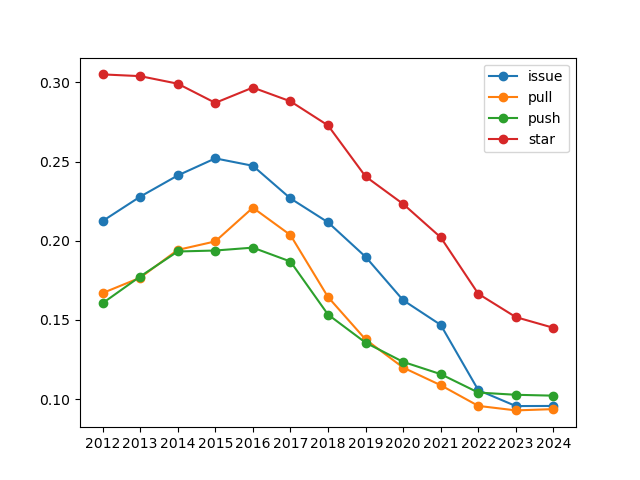
\includegraphics[width=1.0\textwidth]{figures/githut/JavaScript.png}
          \caption{Stats of JavaScript}
        \end{center}
      \end{figure}
    \end{column}
    \begin{column}{0.5\textwidth}
      \begin{figure}
        \begin{center}
          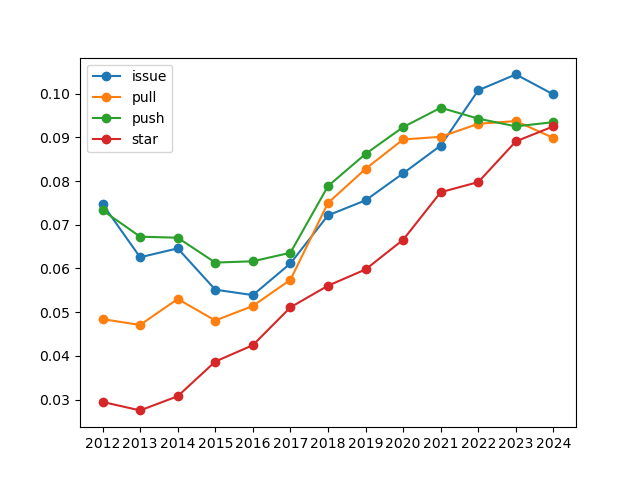
\includegraphics[width=1.0\textwidth]{figures/githut/C++.png}
          \caption{Stats of C++}
        \end{center}
      \end{figure}
    \end{column}
  \end{columns}
\end{frame}

\begin{frame}
  \frametitle{Language Segmentation}
  ... but we can do some estimates
  \begin{figure}
    \begin{center}
      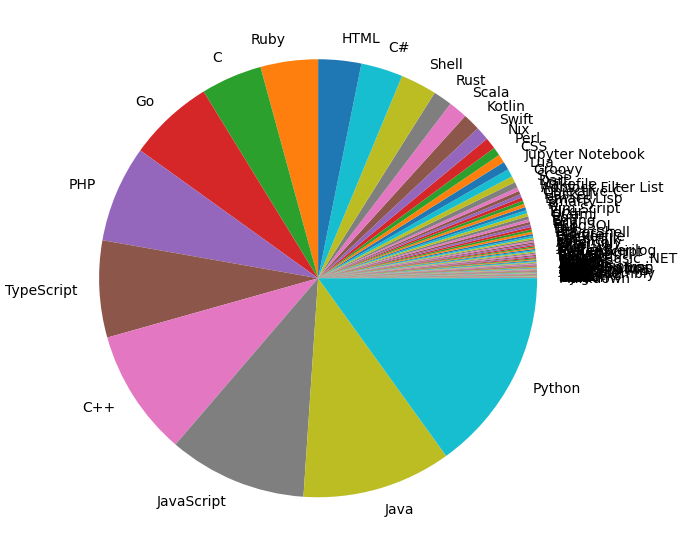
\includegraphics[width=0.8\textwidth]{figures/githut/statistics.png}
    \end{center}
  \end{figure}
\end{frame}

\begin{frame}
  \frametitle{A matter of scale}
  \begin{itemize}
    \item A software analysis tool need to work with many programming languages.
    \item Each deployed instance need every language interface to be useful
    \item Each language interface is a reason to change and increases maintenance costs
  \end{itemize}
  \begin{figure}
    \begin{center}
      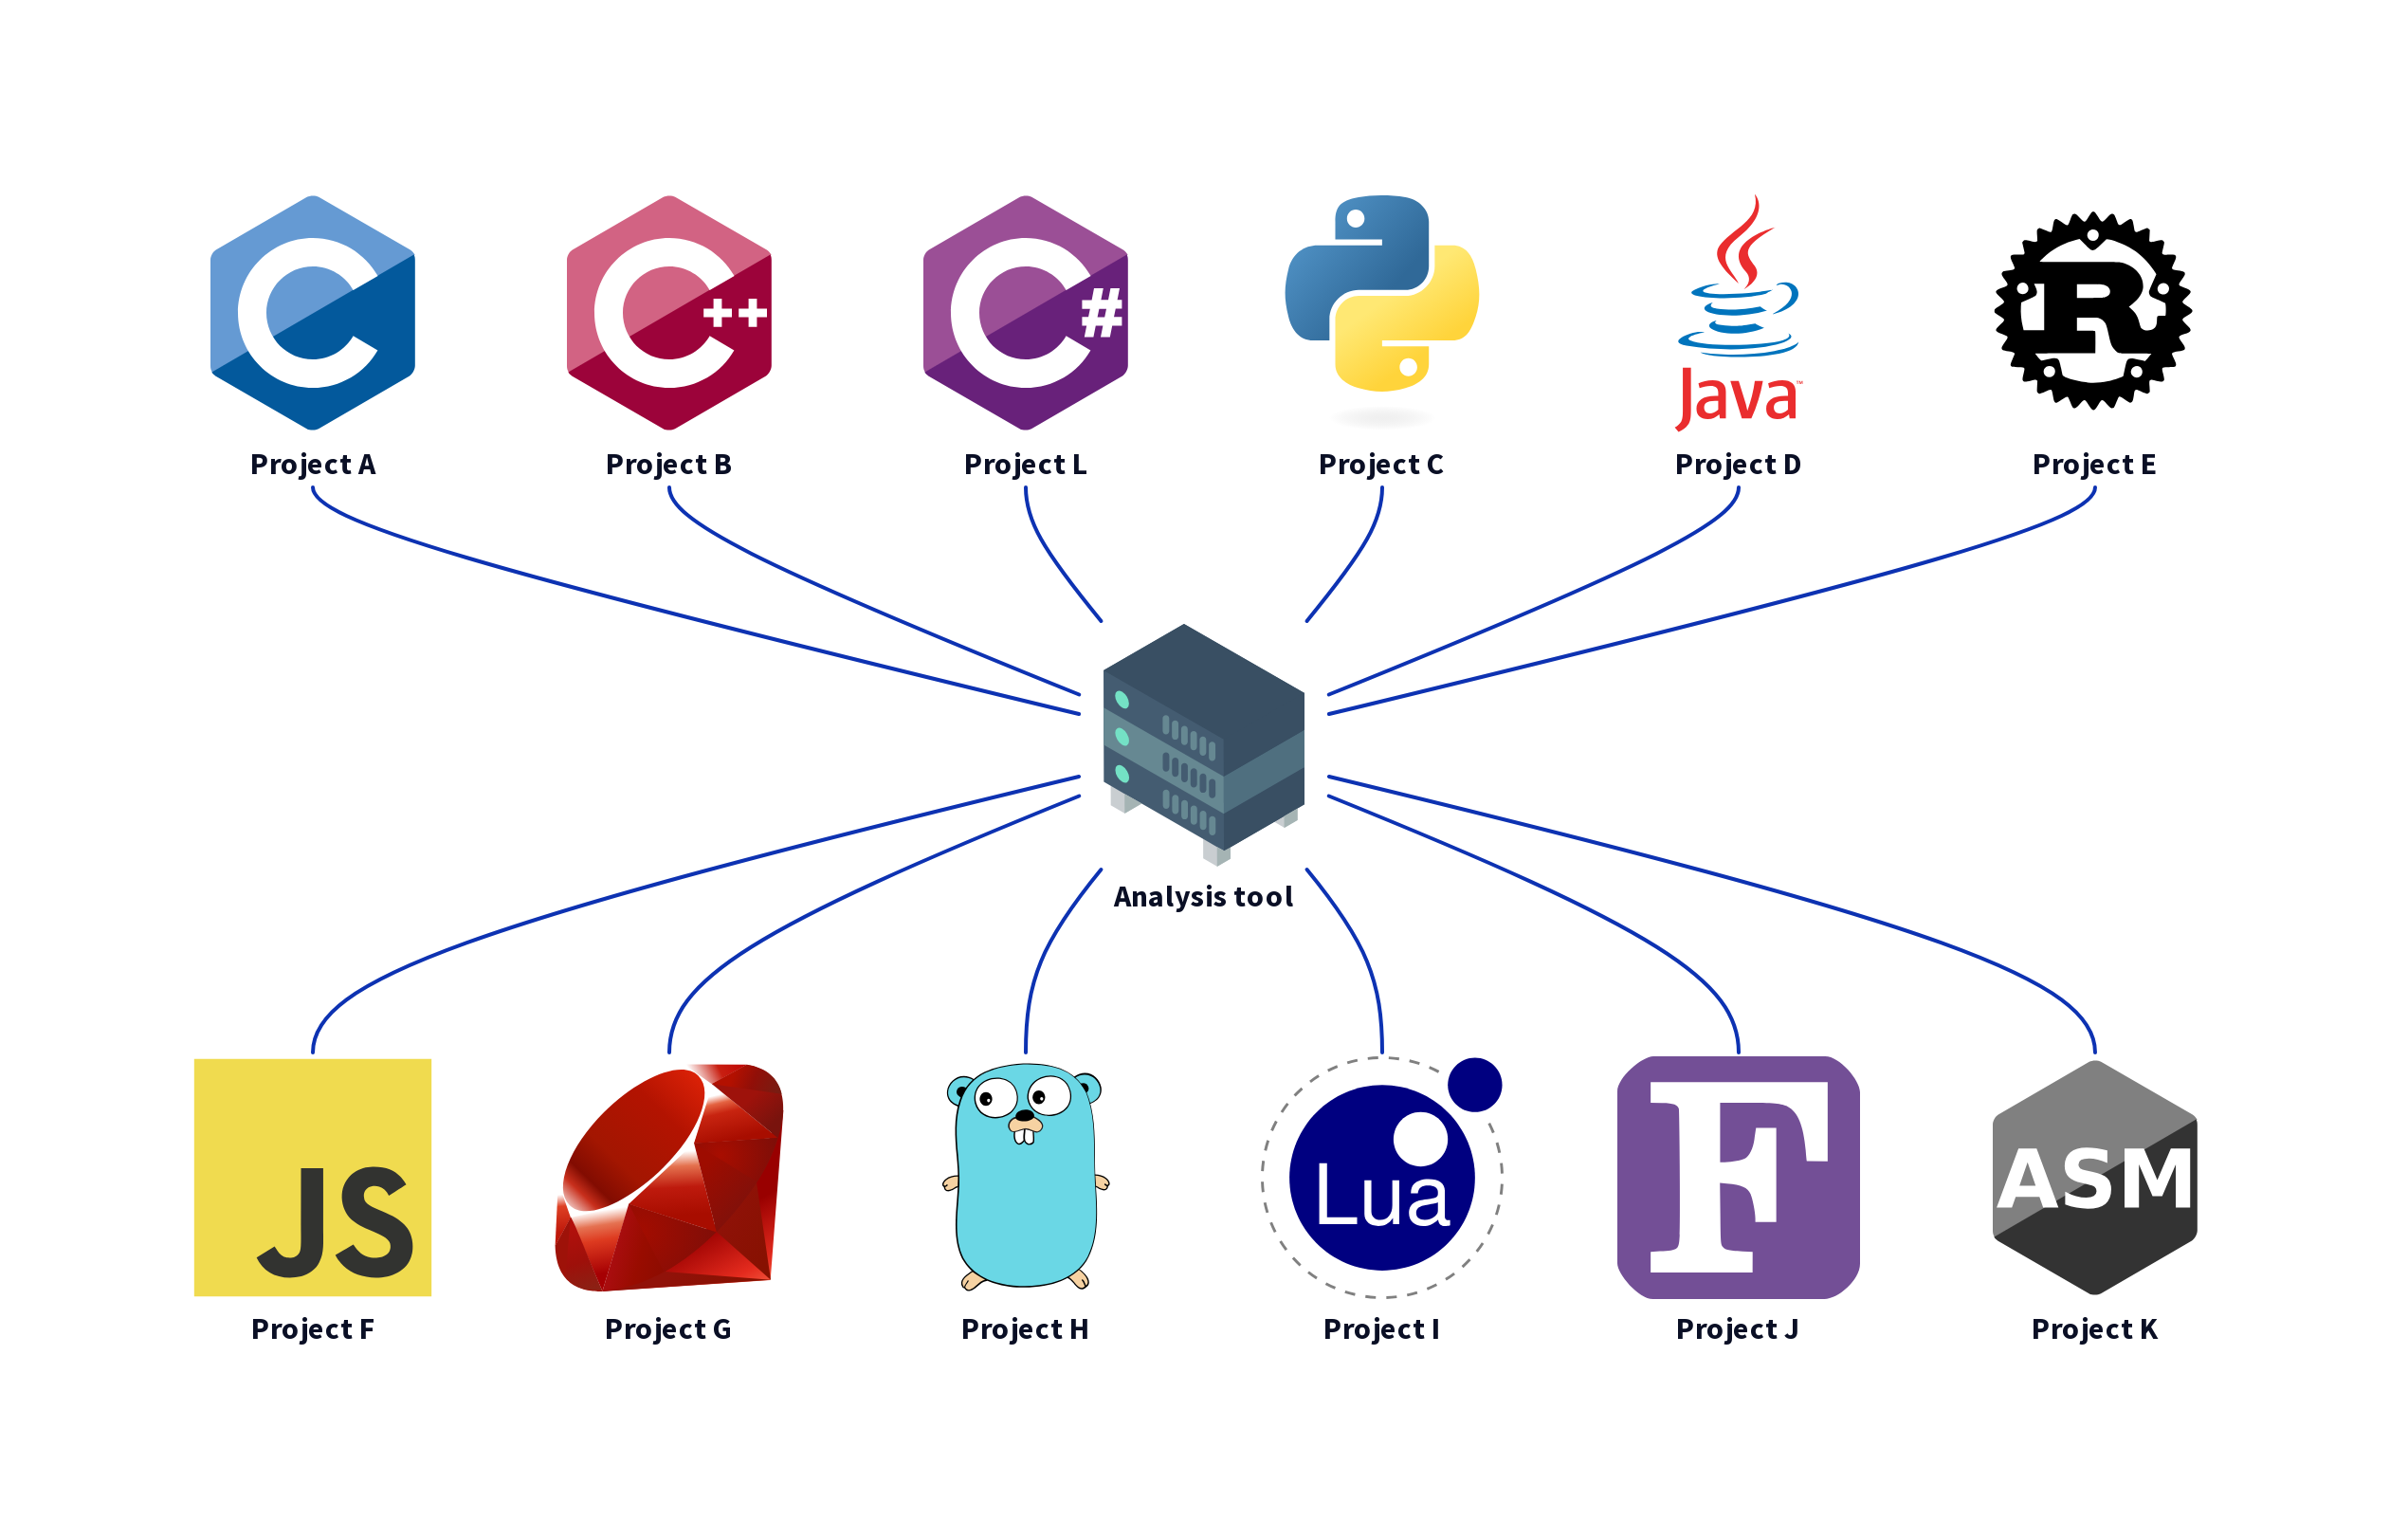
\includegraphics[width=0.7\textwidth]{figures/githut/problem-many-languages.png}
    \end{center}
  \end{figure}
\end{frame}

\begin{frame}
  \frametitle{A matter of perspective}
  \begin{itemize}
    \item A project can use more than one language, which is usually not supported by tools
    \item Each language interface usually need a different implementation for the same logic
    \item Sometimes it is easier to develop a distinct version of each language
  \end{itemize}
  \begin{figure}
    \begin{center}
      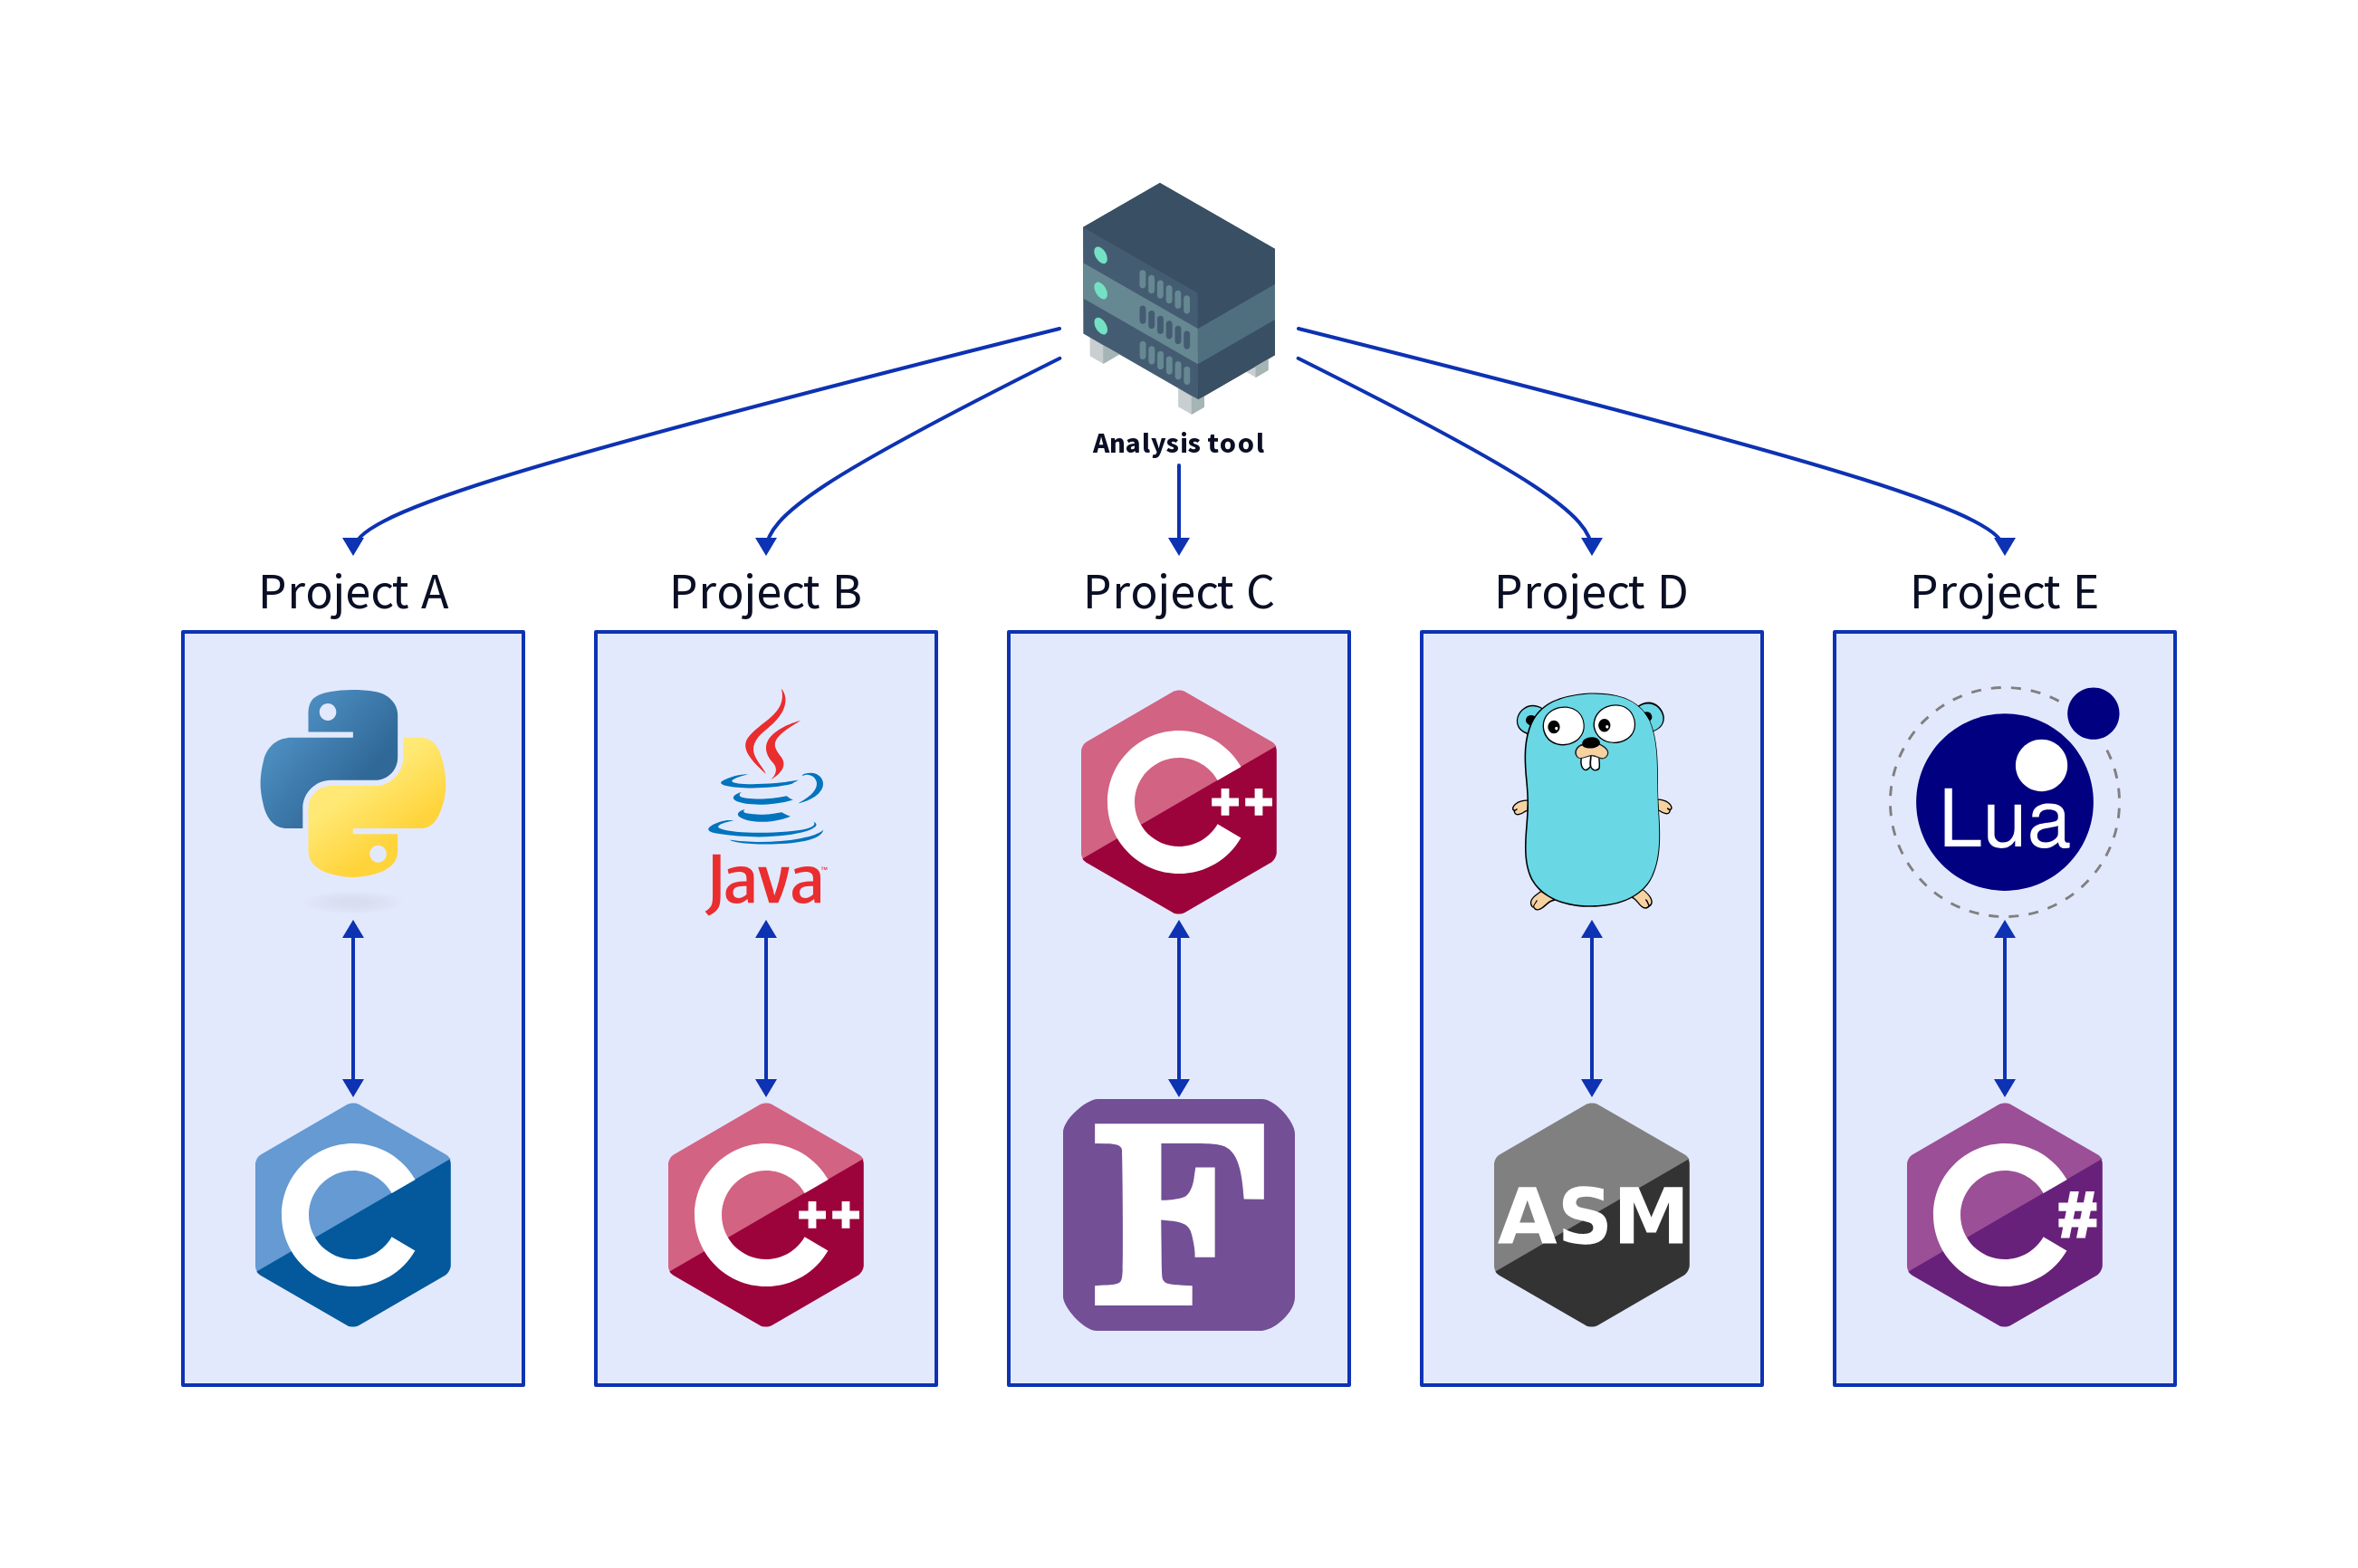
\includegraphics[width=0.7\textwidth]{figures/githut/problem-multi-languages.png}
    \end{center}
  \end{figure}
\end{frame}

\section{A Bit of History}
\begin{frame}
  \centering
  \Huge
  A Bit of History
\end{frame}

\begin{frame}
  \frametitle{Language Frontends}
  \begin{itemize}
    \item Common approach: use language frontends (e.g., \texttt{Clang}, \texttt{Eclipse JDT/CDT}) to parse code and extract data.
    \item APIs are heterogeneous and lack standardization.
    \item The \textit{Language Server Protocol (LSP)} aims to unify such interfaces, but still has limits in query expressiveness and flexibility.
    \item Frontends are designed for IDEs/compilers, requiring extra adaptation for analysis tools.
    \item Typically heavy-weight — include many elaborations not needed by analysis tools.
  \end{itemize}
\end{frame}

\begin{frame}
  \frametitle{Manual/Automatic Transpilation}
  \begin{itemize}
      \item Some works avoid using multiple language frontends by translating source code into a single target language or DSL.
      \item Translation can be done manually or via transpilers.
      \item Works well for languages designed for transpilation (e.g., \texttt{TypeScript}, \texttt{Haxe}).
      \item For other languages, translation may lose semantic details (e.g., classes, namespaces, packages).
      \item To preserve semantics, the target language must be as expressive as the source.
      \item This approach remains inefficient:
      \begin{itemize}
          \item Automatic translation between languages is still an open research problem.
          \item Manual translation is time-consuming and error-prone.
          \item Translated code must still be parsed and analyzed afterward.
      \end{itemize}
  \end{itemize}
\end{frame}

\begin{frame}
  \frametitle{AST/CST Translation}
  \begin{itemize}
      \item Another approach: translate a \textbf{language-dependent AST} into a \textbf{language-independent AST}.
      \item Enables analysis tools to apply algorithms on a common, unified representation.
      \item Can also be applied to \textbf{Concrete Syntax Trees (CSTs)}, which capture full program syntax.
      \item Typically relies on language frontends (manual or generated) to perform near 1:1 translation into an \textit{extended AST (eAST)}.
      \item Sometimes produces an intermediate serialized form (e.g., \texttt{XML}).
  \end{itemize}
\end{frame}

\begin{frame}
  \frametitle{Meta Model Abstraction}
  \begin{itemize}
    \item A \textbf{meta model abstraction} offers a language-agnostic alternative:
    \begin{itemize}
        \item Represents high-level program entities — classes, structs, functions — instead of raw syntax trees.
        \item Simplifies cross-language analysis by focusing on shared structural concepts.
        \item Reduces dependency on language frontends and heavy parsing.
    \end{itemize}
    \item Enables more flexible and extensible analysis frameworks built around \textbf{semantic equivalence} rather than syntax.
    \item Often requires custom frontends to build the meta-model from source code.
  \end{itemize}
\end{frame}

\begin{frame}
  \frametitle{Advanced Data Structures}
  \begin{itemize}
      \item Beyond traditional frontends, new data structures have been designed for specific analysis tasks 
      (e.g., code navigation, reference resolution).
      \item Evaluated the use of \textbf{Stack Graphs} — composable graphs representing identifiers 
      and their relationships — for language-independent reference resolution.
      \item Showed promising accuracy but faced:
      \begin{itemize}
          \item Practical and scalability limitations.
          \item Partial language-independence: graph construction still required language-specific CST queries.
      \end{itemize}
      \item Despite limitations, the study highlighted:
      \begin{itemize}
          \item The potential of \textbf{language-independent analysis}.
          \item Its value as a guiding principle for future software analysis strategies.
      \end{itemize}
  \end{itemize}
\end{frame}

\begin{frame}[fragile]
  \frametitle{ADS / Stack Graphs}
  \begin{columns}
    \begin{column}{0.50\textwidth}
      \begin{itemize}
        \item Composable graph
        \item Represents identifiers and scopes of source code
        \item Enables language agnostic reference resolution
      \end{itemize}
    \end{column}
    \begin{column}{0.50\textwidth}
      \lstinputlisting[language=Java]{listings/stack-graphs/code-example.java}
    \end{column}
  \end{columns}
  \putimage{figures/stack-graphs/stackgraph-example.png}{0.99}
\end{frame}

\begin{frame}[fragile]
  \frametitle{ADS / Tree Sitter Stack Graphs}
  \begin{itemize}
    \item A "TSSG" Grammar is composed of pairs
    \item Each pair matches a section of the CST with some procedural code
    \item Definition of nodes, edges and labels
  \end{itemize}
  \lstinputlisting[style=tssg]{listings/stack-graphs/tssg-example.txt}
\end{frame}

\section{A New Solution}
\begin{frame}
  \centering
  \Huge
  A New Solution
\end{frame}

\begin{frame}[fragile]
  \frametitle{Very different ...}
  \begin{columns}
    \begin{column}{0.5\textwidth}
      \begin{figure}
        \begin{center}
          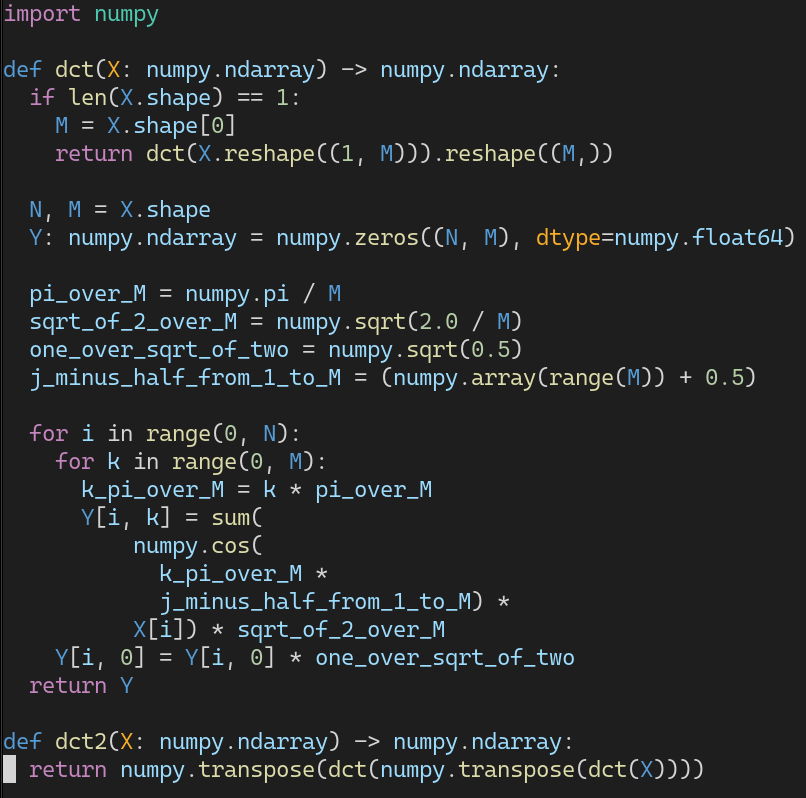
\includegraphics[width=1.0\textwidth]{figures/solution/code-python.png}
        \end{center}
      \end{figure}
    \end{column}
    \begin{column}{0.5\textwidth}
      \begin{figure}
        \begin{center}
          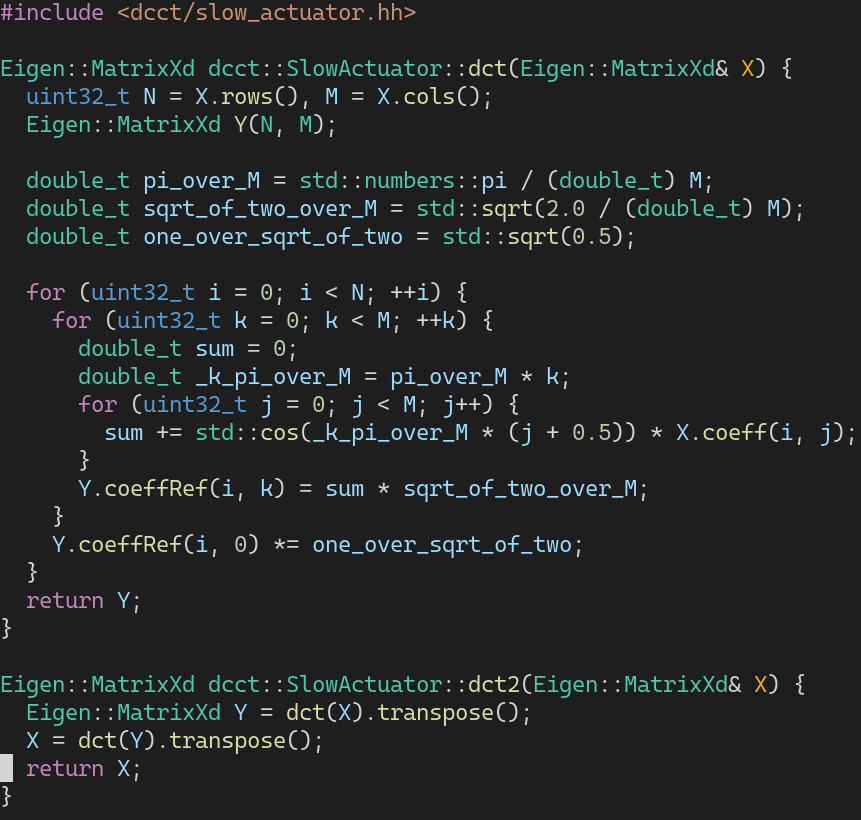
\includegraphics[width=1.0\textwidth]{figures/solution/code-cpp.png}
        \end{center}
      \end{figure}
    \end{column}
  \end{columns}
\end{frame}

\begin{frame}
  \frametitle{... Or very similar?}
  \begin{columns}[T,onlytextwidth]
    \begin{column}{0.5\textwidth}
    \scalebox{0.75}{
    \begin{forest}
      [call\_expression
        [field\_expression
                    [field\_expression
                                [call\_expression
                                            [field\_expression
                                                        [field\_expression
                                                                    [identifier]
                                                                    [field\_identifier]]
                                                        [field\_identifier]]
                                            [argument\_list]]
                                [field\_identifier]]
                    [field\_identifier]]
        [argument\_list]]
    \end{forest}
    }
    \end{column}

    \begin{column}{0.5\textwidth}
    \scalebox{0.75}{
    \begin{forest}
      [call
        [attribute
                    [attribute
                              [call
                                        [attribute
                                                    [attribute
                                                              [identifier]
                                                              [identifier]]
                                                    [identifier]]
                                        [argument\_list]]
                              [identifier]]
                    [identifier]]
        [argument\_list]]
    \end{forest}
    }
    \end{column}
  \end{columns}
\end{frame}

\begin{frame}
  \frametitle{Tree Sitter}
  \begin{columns}
    \begin{column}{0.5\textwidth}
      \begin{figure}
        \begin{center}
          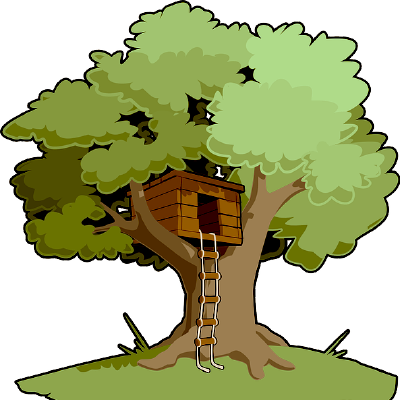
\includegraphics[width=0.5\textwidth]{figures/solution/tree-sitter-logo.png}
        \end{center}
      \end{figure}
    \end{column}
    \begin{column}{0.5\textwidth}
      \begin{itemize}
        \item Tree-sitter is a parser generator tool and an incremental parsing library.
        \item It can build a concrete syntax tree for a source file and efficiently update the syntax tree as the source file is edited.
      \end{itemize}
    \end{column}
  \end{columns}
  \begin{itemize}
    \item General enough to parse any programming language
    \item Fast enough to parse on every keystroke in a text editor
    \item Robust enough to provide useful results even in the presence of syntax errors
    \item Dependency-free so that the runtime library (which is written in pure C11) can be embedded in any application
  \end{itemize}
\end{frame}

\begin{frame}
  \frametitle{Why Tree Sitter?}
  Tree Sitter is not only easy to operate, but it is also easy to implement parsers for new languages.

  \begin{columns}
    \begin{column}{0.5\textwidth}
      \begin{figure}
        \begin{center}
          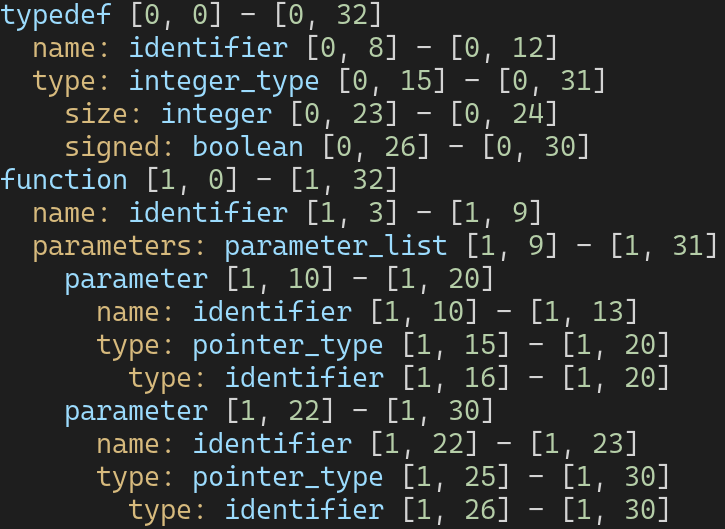
\includegraphics[width=1.0\textwidth]{figures/solution/ts-lart-cst.png}
          \caption{Example of Lart CST}
        \end{center}
      \end{figure}
    \end{column}
    \begin{column}{0.5\textwidth}
      \begin{figure}
        \begin{center}
          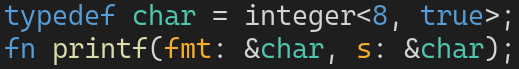
\includegraphics[width=1.0\textwidth]{figures/solution/ts-lart-code.png}
          \caption{Example of Lart code}
        \end{center}
      \end{figure}
      \begin{figure}
        \begin{center}
          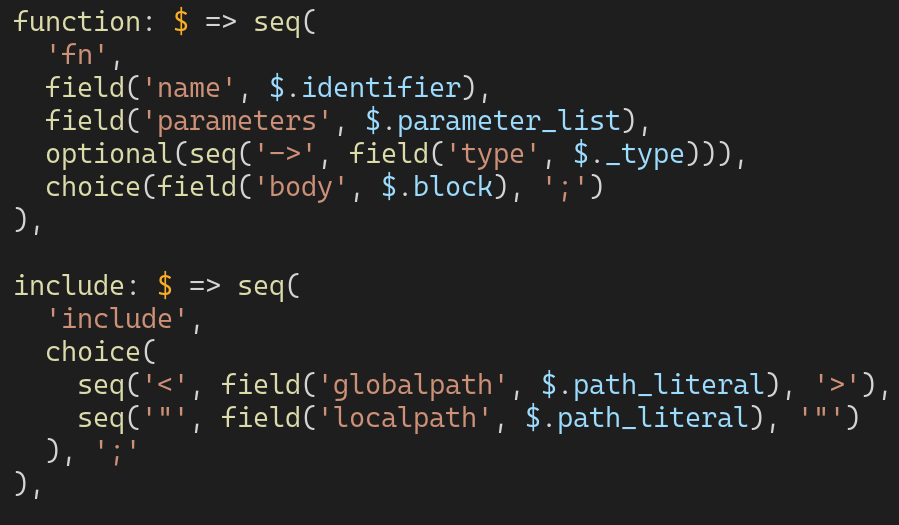
\includegraphics[width=1.0\textwidth]{figures/solution/ts-lart-grammar.png}
          \caption{Slice of Lart grammar as TS config}
        \end{center}
      \end{figure}
    \end{column}
  \end{columns}
\end{frame}

\begin{frame}
  \frametitle{The Approach}
\end{frame}

\begin{frame}
  \frametitle{Why it works}
\end{frame}

\begin{frame}
  \frametitle{Shenanigans}
\end{frame}

\begin{frame}[fragile]
  \frametitle{An Example / The Code}
  \lstinputlisting[language=Java]{listings/approach/code-example.java}
\end{frame}

\begin{frame}
  \frametitle{An Example / The Dependency Graph}
  \putimage{figures/approach/depgraph-example.png}{0.99}
\end{frame}

\section{Evaluation and Comparison}
\begin{frame}
  \centering
  \Huge
  Evaluation and Comparison
\end{frame}

\begin{frame}[fragile]
  \frametitle{The Testing Framework}

  \begin{block}{}
    Tests are described with YAML manifests including constraints on nodes and edges that must be detected in the dependency graph written by the tool
  \end{block}

  \begin{columns}
    \begin{column}{0.64\textwidth}
      \lstinputlisting[style=yaml]{listings/testing/test-manifest-example.yml}
    \end{column}
    \begin{column}{0.34\textwidth}
      \begin{itemize}
        \item node types: class, function, enum ...
        \item edge types: definedBy, includes, usesType, calls ...
      \end{itemize}
    \end{column}
  \end{columns}
\end{frame}

\begin{frame}
  \frametitle{The Dependency Detection Benchmark}
  \begin{figure}
    \begin{center}
      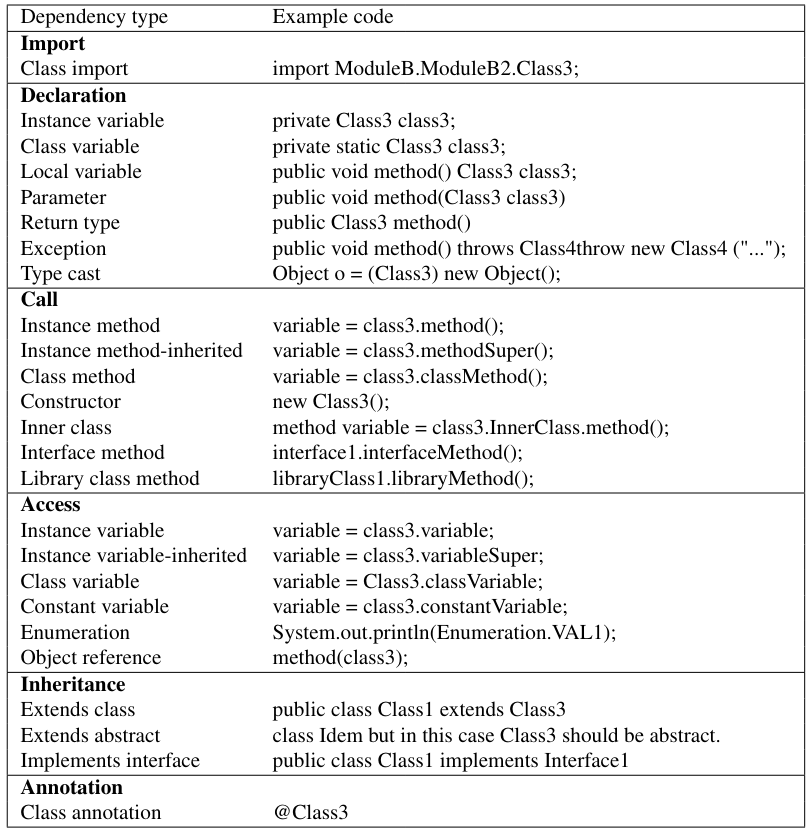
\includegraphics[width=0.6\textwidth]{figures/testing/benchmark-table-1.png}
    \end{center}
  \end{figure}
\end{frame}

\begin{frame}
  \frametitle{The Dependency Detection Benchmark}
  \begin{figure}
    \begin{center}
      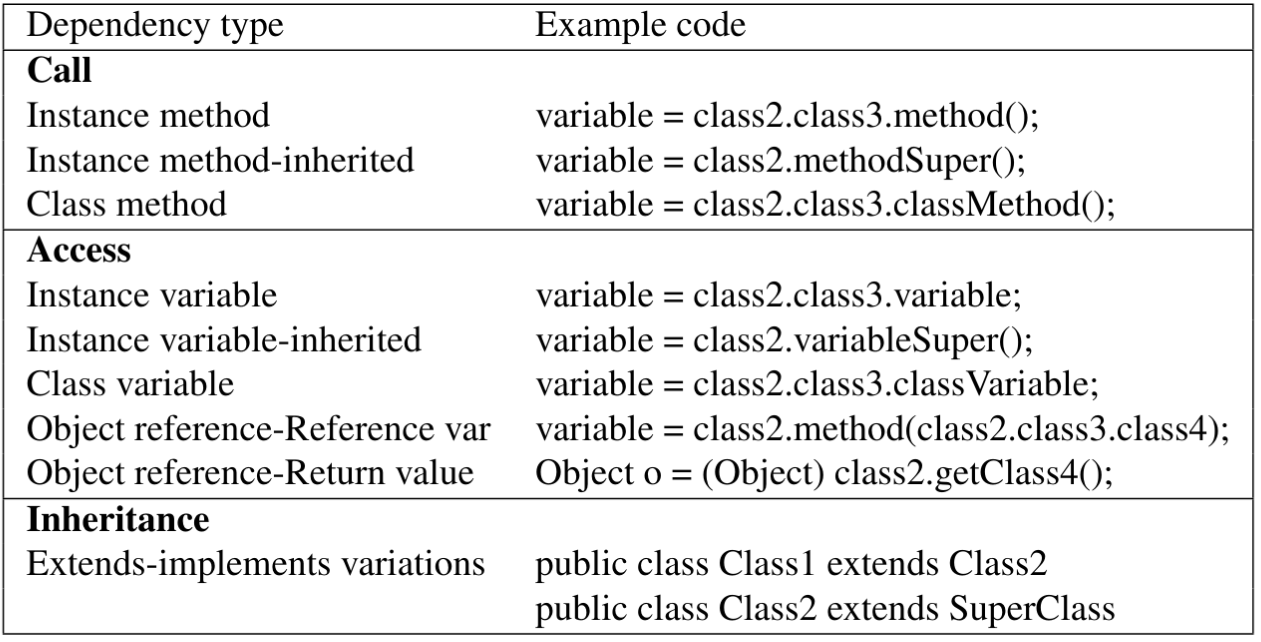
\includegraphics[width=0.9\textwidth]{figures/testing/benchmark-table-2.png}
    \end{center}
  \end{figure}
	\footnote{The accuracy of dependency analysis in static architecture compliance checking, Pruijt et Al, Softw. Pract. Exp. 2017}
\end{frame}

\begin{frame}
  \frametitle{DDB / JAVA}
  \begin{columns}
    \begin{column}{0.3\textwidth}
      \begin{figure}
        \begin{center}
          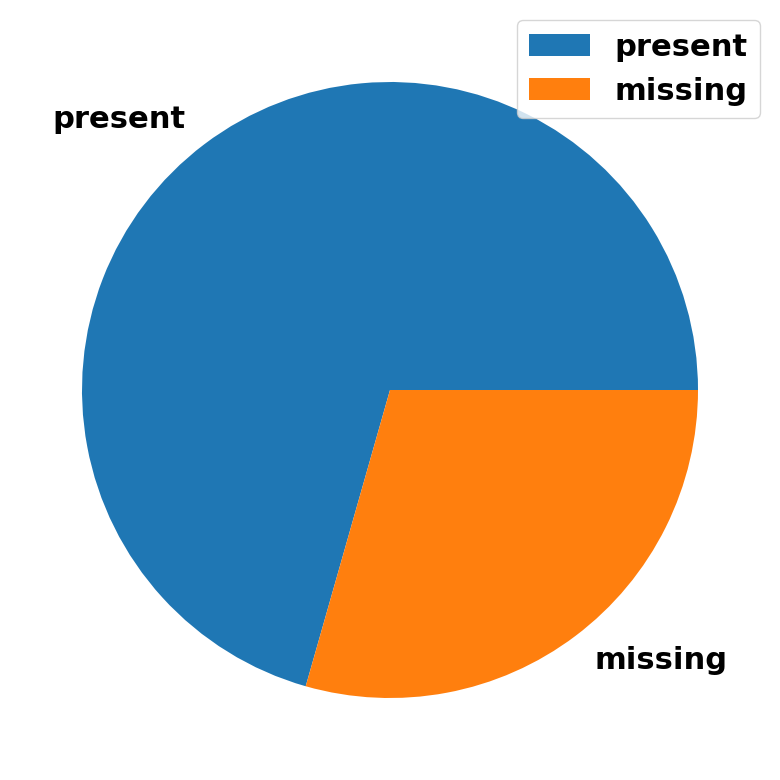
\includegraphics[width=1.0\textwidth]{figures/testing/pie-plot-java-arcan.png}
          \caption{Adherence of Arcan}
        \end{center}
      \end{figure}
    \end{column}
    \begin{column}{0.3\textwidth}
      \begin{figure}
        \begin{center}
          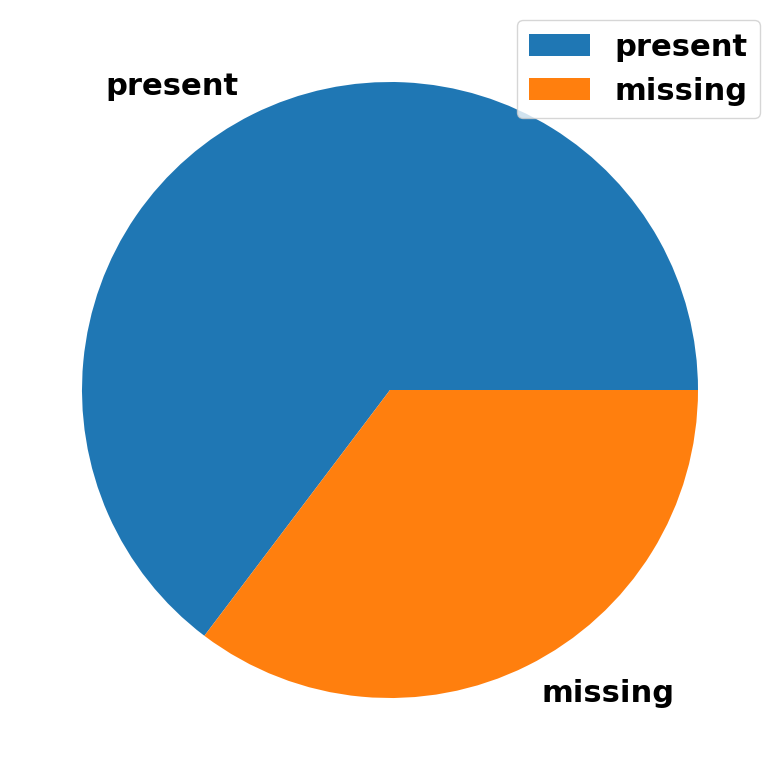
\includegraphics[width=1.0\textwidth]{figures/testing/pie-plot-java-refolli.png}
          \caption{Adherence of the Stack-Graph based solution}
        \end{center}
      \end{figure}
    \end{column}
    \begin{column}{0.33\textwidth}
      \begin{figure}
        \begin{center}
          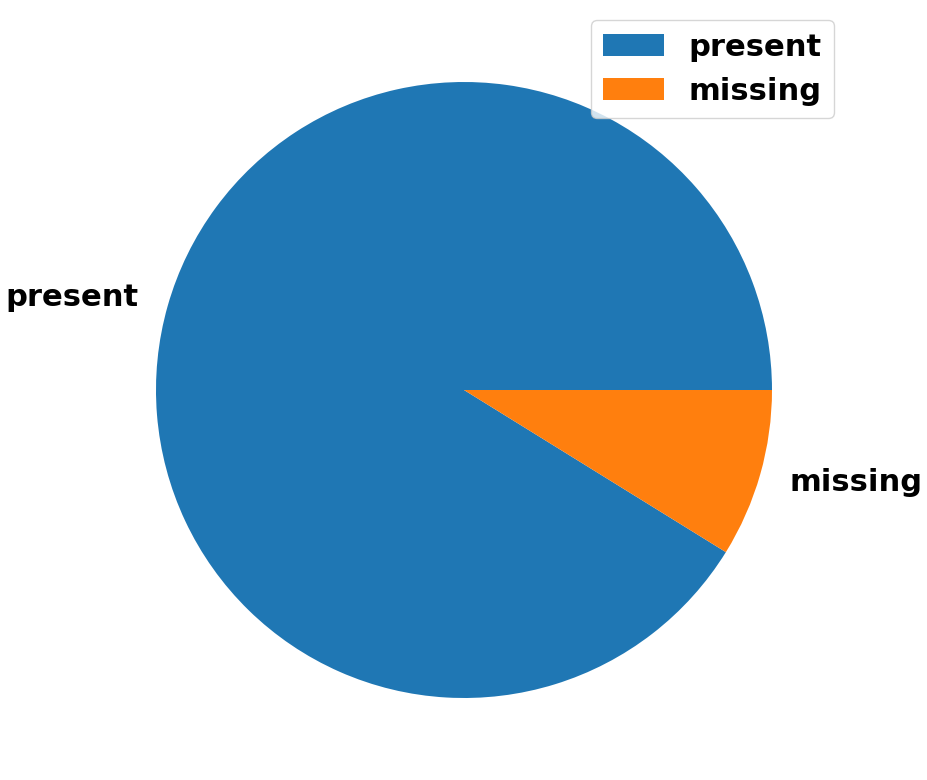
\includegraphics[width=1.0\textwidth]{figures/testing/pie-plot-java-teruzzi.png}
          \caption{Adherence of the new proposed solution}
        \end{center}
      \end{figure}
    \end{column}
  \end{columns}
\end{frame}

\begin{frame}
  \frametitle{DDB / JAVA}
  \begin{figure}
    \begin{center}
      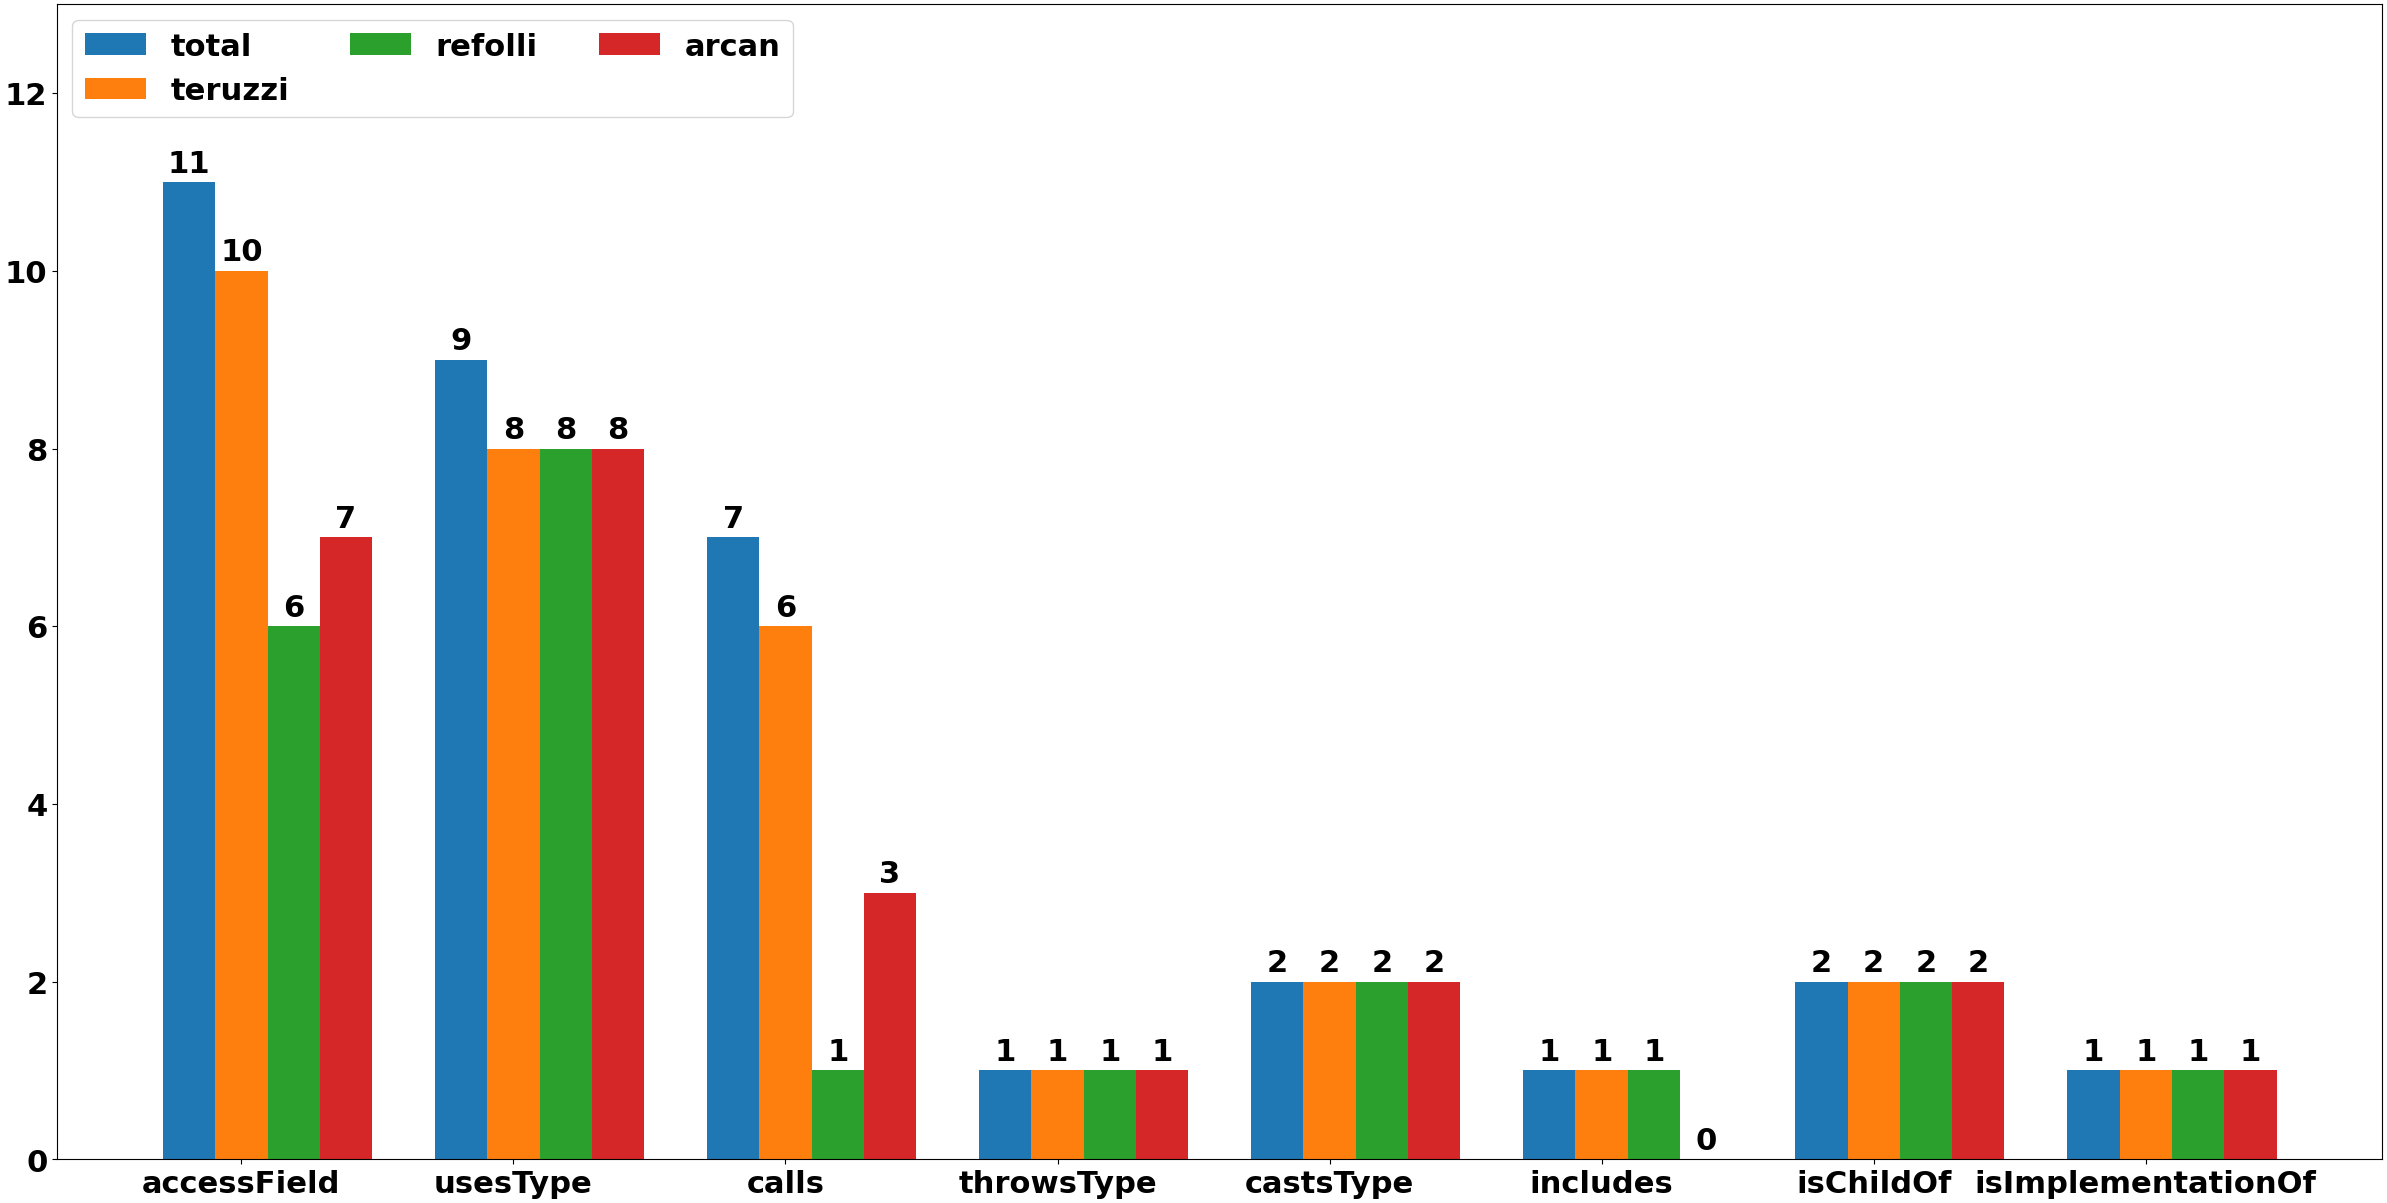
\includegraphics[width=1.0\textwidth]{figures/testing/bar-plot-java.png}
    \end{center}
  \end{figure}
\end{frame}

\begin{frame}
  \frametitle{DDB / RUST}
  \begin{figure}
    \begin{center}
      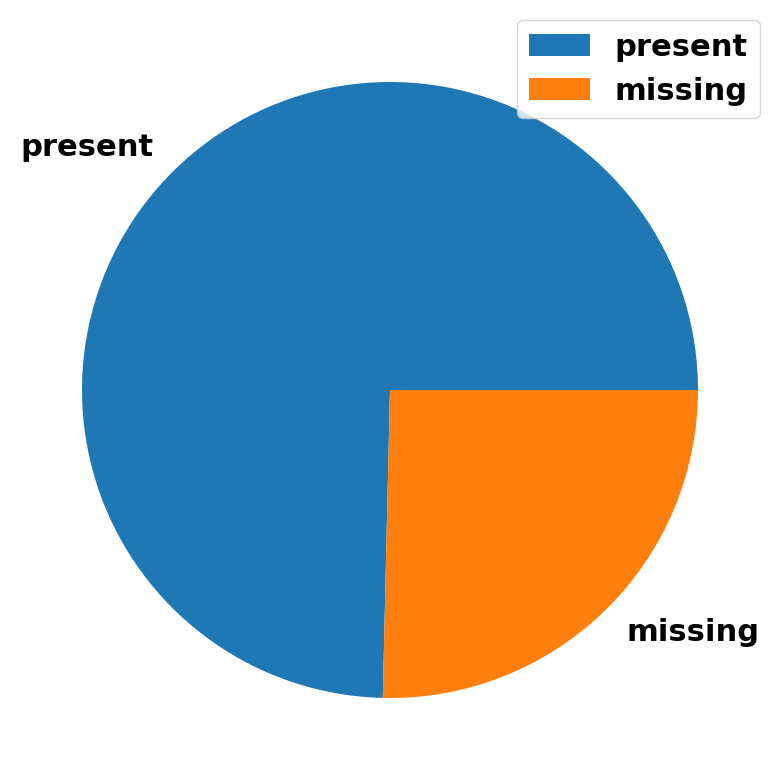
\includegraphics[width=0.7\textwidth]{figures/testing/pie-plot-rust-teruzzi.png}
      \caption{Adherence of the new proposed solution}
    \end{center}
  \end{figure}
\end{frame}

\begin{frame}
  \frametitle{DDB / RUST}
  \begin{figure}
    \begin{center}
      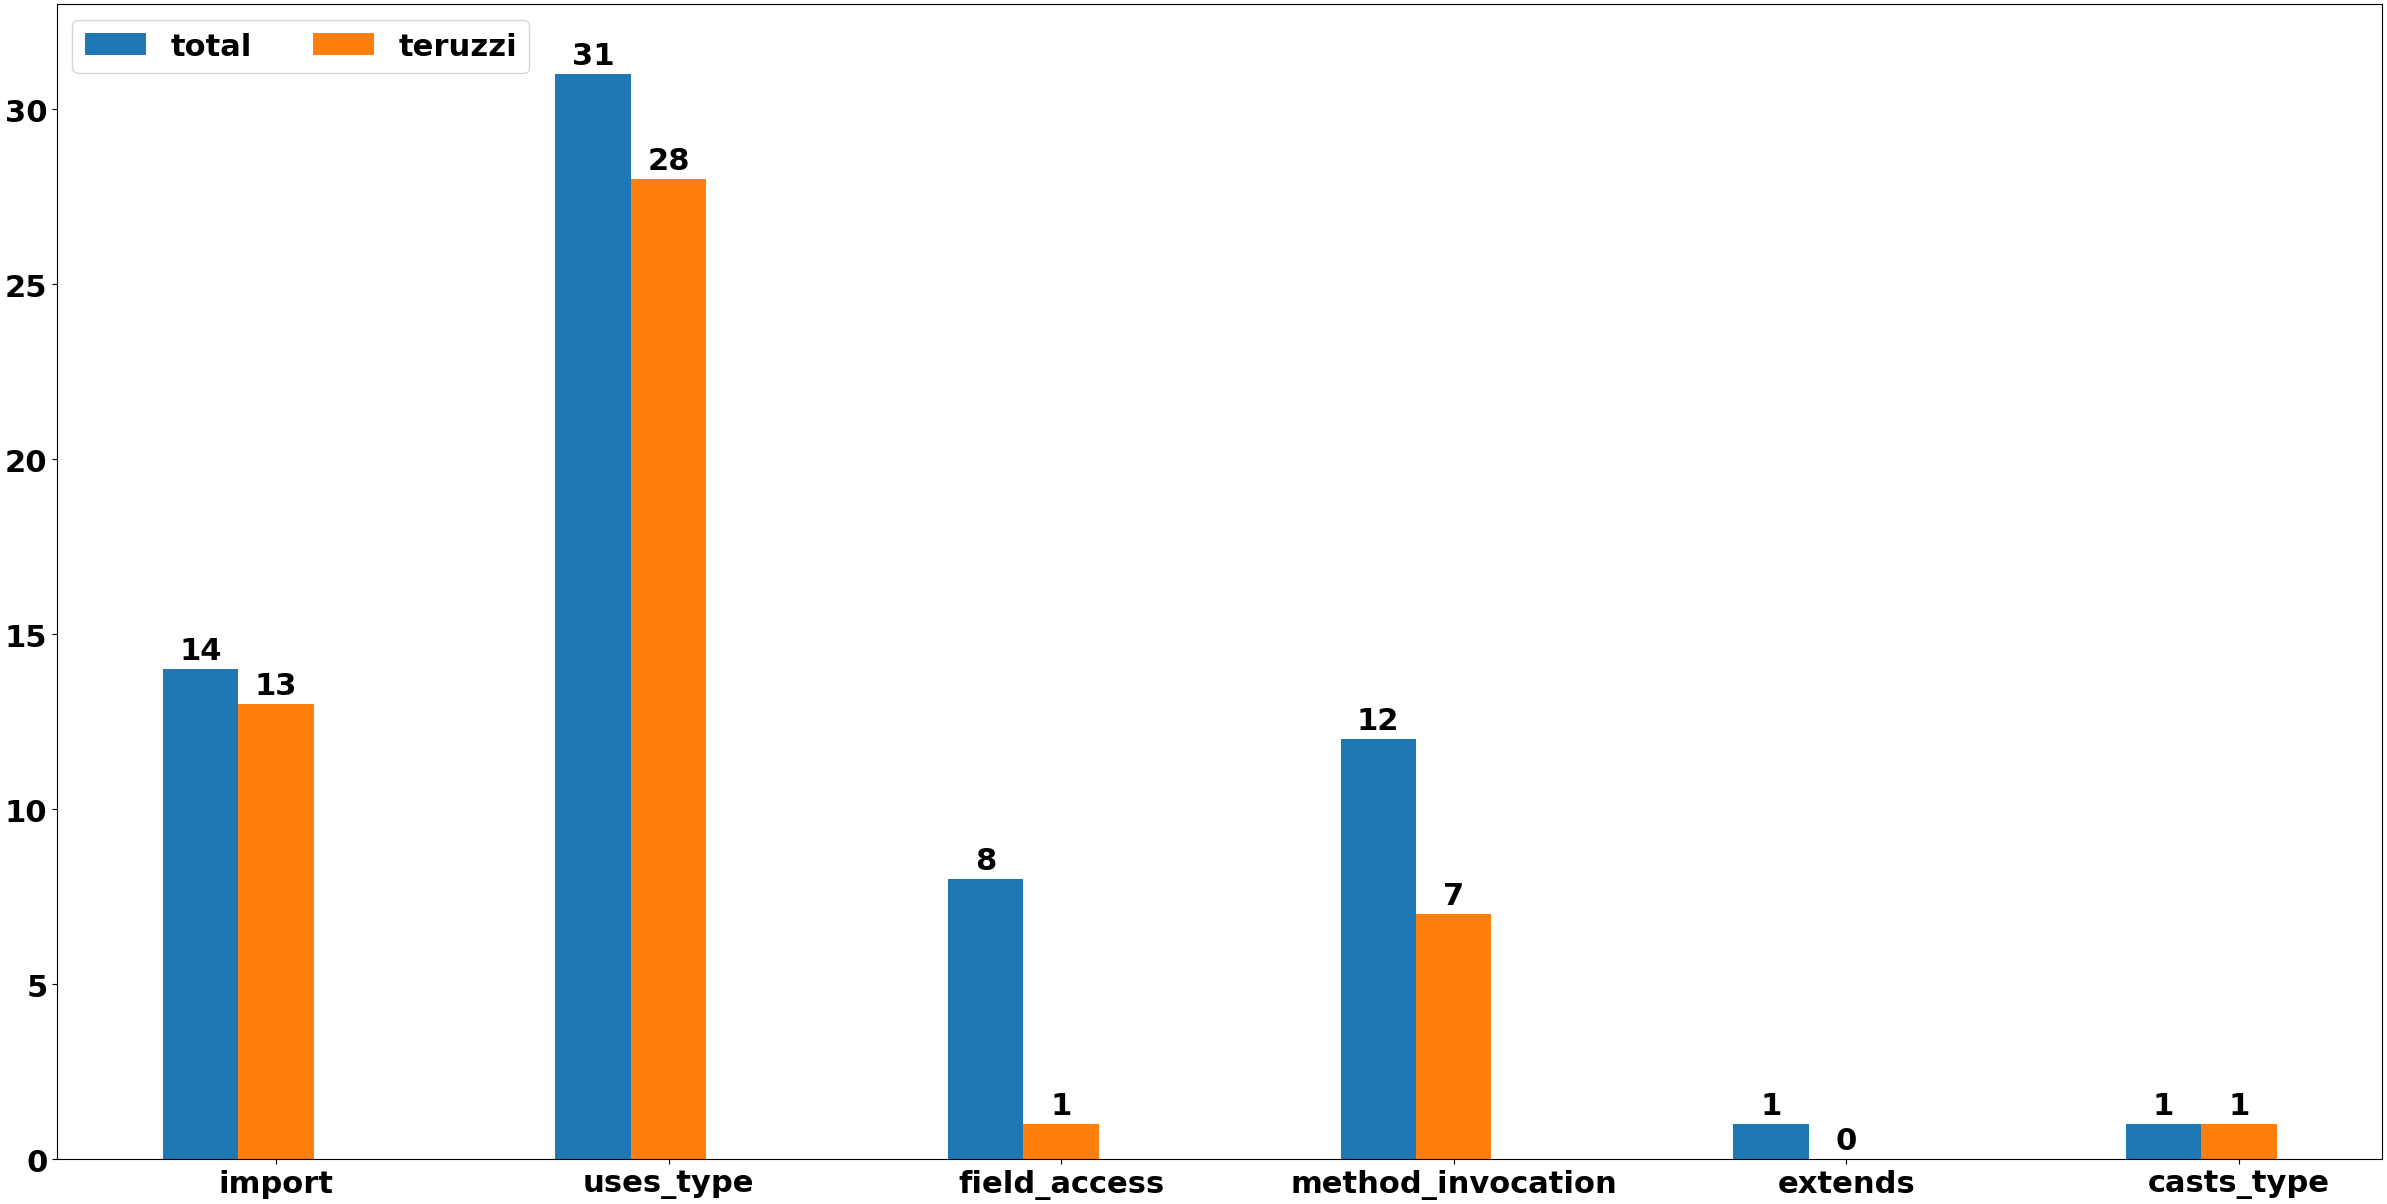
\includegraphics[width=1.0\textwidth]{figures/testing/bar-plot-rust.png}
    \end{center}
  \end{figure}
\end{frame}

\begin{frame}
  \frametitle{Comparison with the previous iteration}

  \begin{block}{}
    \begin{itemize}
      \item The Stack-Graph based solution had a decent effectiveness when dealing with small scale projects, but efficiency is another story.
      \item In some cases it didn't even complete the scan within a reasonable time.
      \item For these reasons, the comparison is drawn mainly with Arcan in the next slides.
    \end{itemize}
  \end{block}
  
  \center
  \begin{tabular}{|l|l|l|l|l|}
      \hline
      \textbf{Project} & \textbf{Tool} & \textbf{Min} & \textbf{Max} & \textbf{Mean execution time} \\ \hline
      \hline
      \rowcolor[HTML]{EED49F} 
      JUnit4   & Stack-Graph & 65,82  & 69,07  & 65,88     \\ \hline
      \rowcolor[HTML]{A6DA95} 
      JUnit4   & Arcan     & 13,850 & 17,079 & 14,611    \\ \hline
      \rowcolor[HTML]{EED49F} 
      JUnit5   & Stack-Graph & 132,87 & 134,75 & 134,44    \\ \hline
      \rowcolor[HTML]{A6DA95} 
      JUnit5   & Arcan     & 42,542 & 47,613 & 44,186    \\ \hline
      \rowcolor[HTML]{EED49F} 
      ANTLR    & Stack-Graph & 171,65 & 175,49 & 172,64    \\ \hline
      \rowcolor[HTML]{A6DA95} 
      ANTLR    & Arcan     & 19,222 & 20,140 & 19,691    \\ \hline
      \rowcolor[HTML]{ED8796} 
      Fastjson & Stack-Graph & N/A    & N/A    & N/A       \\ \hline
      \rowcolor[HTML]{A6DA95} 
      Fastjson & Arcan     & 66,932 & 71,094 & 69,071    \\ \hline
  \end{tabular}
\end{frame}

\begin{frame}
  \frametitle{Comparison with Arcan / Accuracy}
\end{frame}

\begin{frame}
  \frametitle{Comparison with Arcan / Similarity}
\end{frame}

\begin{frame}
  \frametitle{Comparison with Arcan / Efficiency}
\end{frame}

\section{Conclusions}
\begin{frame}
  \centering
  \Huge
  Conclusions
\end{frame}

\begin{frame}
  \frametitle{Open Problems}
\end{frame}

\begin{frame}
  \frametitle{Future Works}
\end{frame}

\begin{frame}[allowframebreaks, noframenumbering]
\frametitle{Bibliography}
\printbibliography
\nocite{*}
\end{frame}

\end{document}
